\documentclass[12pt,a4paper]{article}
%\documentclass[oribibl]{llncs}
%\usepackage{subfigure}

%\documentclass[12pt]{tesis}

\usepackage{verbatim} % Para incluir comentarios que abarquen varias l�neas
\usepackage[latin1]{inputenc} % Para acentos
\usepackage[spanish]{babel} % Titulos en castellano
\usepackage{hyperref}
\usepackage{array}
\usepackage[pdftex]{graphicx}
\usepackage[font=small,format=plain,labelfont=bf,up,textfont=it,up]{caption} % Letra de los comentarios de las imagenes
%\usepackage{sidecap}

\setcounter{secnumdepth}{5} % profundidad de las secciones

\DeclareGraphicsExtensions{.pdf,.png,.jpg}

%\author{Virginia Arroyo, Juli�n Oyola \\ \normalsize \emph{Facultad de Ciencias Exactas y Naturales, Universidad de Buenos Aires}}
%\principaladviser{Ana Ruedin y Daniel Acevedo}

\title{}
\date{}

\begin{document}

%\oddsidemargin 0in %dice al compilador de Latex que el m�rgen izquierdo ser� de 1+0 pulgadas desde el borde izquierdo de la hoja
%\textwidth 7.75in %define el ancho del texto y con esto tambi�n se puede calcular el m�rgen derecho asociado
%\topmargin 0 %coloca el margen superior del texto a 1+0 pulgadas desde el inicio de la hoja.
%\headheight 0in %define el largo del texto excluyendo el encabezado y el pie de p�gina.
%\textheight 8.5in %largo del texto

\maketitle






\vspace{3cm}


\begin{center}
\thispagestyle{empty}


\

\

\

\

\hspace{-5cm} % para dvi
\special{bmp: uni.bmp x=2 y=2}


\

{\Large {\sc Tesis de Licenciatura}}\\

\

\

{\Large {\sc Departamento de Computaci�n}}\\
\vspace{2mm}
{\Large {\sc Facultad de Ciencias Exactas y Naturales}}\\
\vspace{2mm}
{\Large {\sc Universidad de Buenos Aires}}\\

\

\

 

{\Large {\bf Tema: An�lisis y extracci�n de caracter�sticas de enfermedades de la piel: su aplicaci�n en la detecci�n de varicela}}\\ 

\

\

\


{\Large Alumnos: Juli�n Oyola y Virginia Arroyo}\\
\vspace{1mm}
{\Large Directora: Dra. Ana Ruedin}\\
\vspace{1mm}
{\Large Codirector: Dr. Daniel Acevedo}\\


\end{center}

\break
\chapter*{\runtitulo}

\small

\emph{
Las t�cnicas de procesamiento de im�genes pueden resultar de ayuda a los profesionales de la medicina en el diagn�stico temprano de enfermedades de la piel. Este trabajo se centra en el an�lisis y extracci�n de caracter�sticas propias de la varicela sobre fotograf�as digitales del paciente, y en la comparaci�n de las mismas con enfermedades similares.
El procedimiento utilizado para la detecci�n consiste en el an�lisis de la luminancia, el mejoramiento del contraste por medio de la ecualizaci�n del histograma, la suavizaci�n de la imagen y la detecci�n de bordes. Luego aplicamos operaciones morfol�gicas sobre los bordes hallados y la transformada de Hough para detectar los c�rculos de las ves�culas de la varicela. De esta forma se consigue, para un conjunto representativo de im�genes, un m�todo de detecci�n de ves�culas de la varicela con una tasa razonable de aciertos.
Una vez aplicada la detecci�n, realizamos un an�lisis comparativo de los histogramas de color de las ves�culas, centr�ndonos en m�todos num�ricos que permitan distinguir elementos reales de falsos positivos, y tambi�n distinguir ves�culas de varicela de las de otra enfermedad, como el herpes z�ster, obteni�ndose resultados altamente satisfactorios.
Por �ltimo, realizamos un an�lisis sobre las medias de los colores de las ves�culas de varicela y piel sana, como as� tambi�n entre ves�culas de varicela y herpes z�ster, encontrando diferencias alentadoras que podr�an ser utilizadas para la discriminaci�n entre piel sana y varicela, o entre varicela y otra enfermedad. 
}

\paragraph{Palabras clave:}

Transformada de Hough circular, detecci�n de ves�culas de varicela, filtro gaussiano, espacios de color, Kullback-Leibler Divergence, distancia Mahalanobis.




\section {Introducci�n}

La varicela es una enfermedad causada por el virus de la varicela z�ster, un virus de la familia de los herpesvirus. La varicela es muy contagiosa y se desarrolla principalmente en ni�os. El virus se transmite generalmente por v�a a�rea, por medio de las gotas de Fl�gge (peque�as gotitas que expelen los pacientes al respirar), y tambi�n por contacto directo, aunque en menor medida. Tiene un per�odo de incubaci�n de 10 a 21 d�as y durante �l no se presentan s�ntomas hasta que aparecen las primeras lesiones en la piel en forma de peque�os granos, que se presentan de forma s�bita y evolucionan el pocas horas pasando de manchas a lesiones sobreelevadas en la piel que se conocen como p�pulas, que despu�s se llenan de l�quido formando ves�culas. Posteriormente se llenan de pus y se conocen como p�stulas que por �ltimo forman costras. Despu�s del periodo de incubaci�n, aparecen los primeros s�ntomas que son fiebre no muy alta, malestar general y unas peque�as p�pulas rojizas. La erupci�n aparece primero en el abdomen y la espalda, y luego, se propaga a casi todas las partes del cuerpo, incluidos el rostro, el cuero cabelludo, la boca, la nariz, las orejas y los genitales. Las ves�culas de la varicela suelen medir menos de un cent�metro de ancho, tienen una base roja y aparecen en tandas o brotes en el transcurso de dos a cuatro d�as. Lo habitual es que aparezcan de 3 a 4 brotes. Por lo general, la varicela es una enfermedad leve, pero puede ser grave en embarazadas, lactantes, adolescentes, adultos y personas con sistemas inmunitarios debilitados.

Luego de la infecci�n, el virus de la varicela z�ster puede quedar latente dentro de los nervios perif�ricos del cuerpo, sin causar ning�n s�ntoma. D�as o d�cadas m�s tarde, el virus puede activarse nuevamente, saliendo de las c�lulas nerviosas y formando nuevas ves�culas en la piel, en forma de anillo agrupadas a lo largo de un dermatoma (el �rea de la piel inervada por una ra�z o nervio dorsal de la m�dula espinal). A esta nueva aparici�n del virus se la conoce como herpes z�ster (o culebrilla) y suelen padecerla personas con un sistema inmunol�gico debilitado. Cuando aparece la culebrilla, s�lo afecta un lado del cuerpo, usualmente tiene el aspecto de una franja, como un cintur�n a lo largo de una �nica l�nea o filamento nervioso. El sitio donde aparece con m�s frecuencia es la espalda, en la parte superior del abdomen o en la cara. Los primeros signos del herpes z�ster son fiebre, escalofr�os, fatiga, dolor de cabeza y malestar estomacal, lo cual puede confundir a la gente, creyendo que est�n con una gripe. Estos s�ntomas habitualmente est�n acompa�ados de una sensaci�n de hormigueo, adormecimiento o dolor en un lado del cuerpo o de la cara. Muchas personas describen el dolor como una quemaz�n, pulsaciones y un dolor punzante, con puntadas agudas e intermitentes de mucho dolor. Algunas personas experimentan una picaz�n severa o molestias m�s que un verdadero dolor. Luego de varios d�as con estos s�ntomas, aparece una erupci�n en forma de franja como un cintur�n que se extiende desde la l�nea media del cuerpo hacia afuera. La erupci�n aparece como un peque�o grupo de ampollas en forma de uvas, llenas de un l�quido claro sobre una piel enrojecida. Dentro de los tres d�as posteriores a la erupci�n, las ampollas se tornan amarillas, se secan y se forman costras. El herpes z�ster no se puede transmitir a alguien que haya tenido varicela en el pasado o haya sido vacunado para evitar la infecci�n con el virus de la varicella zoster. Alguien que no haya padecido la varicela o que no se haya vacunado, puede desarrollar varicela si toma contacto con un brote de herpes z�ster. Aproximadamente, entre el 3 por ciento y el 5 por ciento de las personas infectadas con el virus de la varicela zoster padecer�n herpes z�ster en alg�n momento de sus vidas, la mayor�a de ellas despu�s de los 50 a�os de edad.

El objetivo principal de este trabajo consiste en desarrollar un m�todo capaz de detectar ves�culas de varicela, y analizar sus caracter�sticas en forma comparativa con otras enfermedades. Para obtenerlo trabajamos con t�cnicas de reconocimiento de patrones.

Entre los temas m�s importantes en el procesamiento de im�genes digitales se encuentra el reconocimiento de patrones, debido a que est� relacionado con la identificaci�n de objetos. Este tema se ha tratado con distintos enfoques y t�cnicas, como puede apreciarse en trabajos tales como el de Flores y M�ndez ~\cite{AF01} del a�o 2009, que utiliza la segmentaci�n de im�genes y la detecci�n de bordes por Canny para encontrar los bordes de una oreja, o el trabajo de Rizon et al.\ ~\cite{CH01}, que utiliza t�cnicas de segmentaci�n y la transformada circular de Hough o CHT (Circular Hough Transform), para detectar el contorno de cocos en una imagen. En visi�n artificial se han desarrollado m�todos para seguimiento trayectorias utilizando la transformada de Hough y el filtrado de Canny ~\cite{JJ01}. En cuanto al reconocimiento de objetos se ha propuesto m�todos para distinguir el ojo de una persona y poder realizar la medici�n del di�metro del iris ~\cite{BC01} utilizando Canny y CHT. Por otro lado, en im�genes satelitales se presentaron publicaciones donde se explica c�mo determinar la edad geol�gica de cr�teres en Marte utilizando como principales herramientas la detecci�n de bordes (Canny) y de c�rculos (CHT)~\cite{AF01}. Finalmente podemos mencionar un sistema biom�trico de reconocimiento del iris utilizando una c�mara convencional para la captura de im�genes propuesto en el art�culo ~\cite{TC01}, que presenta un m�todo que aplica Canny y luego CHT para luego normalizar el resultado de manera tal que el mismo puede ser comparado con otra captura. 

Para detectar las ves�culas de varicela y analizar sus caracter�sticas, aplicamos distintas metodolo g�as, de acuerdo a los resultados que deseabamos obtener. En la etapa de preprocesamiento de la imagen, trabajamos con distintos espacios de color, hasta hallar el adecuado para cada una de las etapas posteriores. Tambi�n en esta etapa debimos mejorar el contraste de las im�genes para prepararlas para la siguiente etapa. En la etapa de an�lisis de formas, probamos con varios m�todos la detecci�n de bordes, qued�ndonos con el m�todo que en la bibliografia recomienda como m�s robusto; y que luego durante las pruebas result� adecuado. El m�todo de detecci�n de bordes elegido fue el m�todo Canny ~\cite{JC01}. Adem�s en esta etapa debimos detectar la forma circular de las ves�culas de varicela. Para esta detecci�n utilizamos la Transformada Circular de Hough ~\cite{DH01} ~\cite{SJ01}. En la �ltima etapa trabajamos en la obtenci�n de caracter�sticas de las ves�culas de varicela y de herpes para poder identificar, a trav�s de esas caracter�sticas, las im�genes que contengan ves�culas de varicela o herpes, como as� tambi�n poder determinar regiones de piel sana y regiones con ves�culas. Para ello utilizamos los histogramas de color de las ves�culas en distintos espacios de color y los comparamos con diferentes m�todos, tanto sim�tricos: distancias o normas, como no sim�tricos como el KLD (Kullback Leibler divergence). Tambi�n analizamos las medias de las ves�culas de varicela y de herpes, utilizando diferentes tests, que nos permiten aproximarnos a la extracci�n de caracter�sticas que puedan ayudar en la identificaci�n de regiones de la imagen que contengan ves�culas de la enfermedad estudiada. Elegimos im�genes de herpes z�ster para comparar con las im�genes de varicela; y de esta forma evaluar como se comporta el procedimiento propuesto, dado que ambas enfermedades causan lesiones similares en la piel.

En el curso de esta tesis hemos presentado dos trabajos, una presentaci�n en un congreso nacional ~\cite{JO02} y otra en un congreso internacional ~\cite{JO01}.

A continuaci�n se describe c�mo se encuentra organizado el presente trabajo. En la secci�n 2 hablamos de las im�genes utilizadas y de sus propiedades. En la secci�n 3 detallamos los m�todos que utilizamos para detectar ves�culas (ecualizaci�n del histograma, selecci�n del espacio de color, m�todo Canny, transformada circular de Hough, entre otros). En la secci�n 4 explicamos como discriminamos entre ves�culas de varicela y ves�culas de otras enfermedades como el herpes, utilizando histogramas de las componentes de color y analiz�ndolos a trav�s de la norma y la divergencia KLD. En la misma secci�n, analizamos las medias de las componentes de color de las ves�culas de varicela y las comparamos con piel sana y con ves�culas de herpes. En la secci�n 5 damos las conclusiones finales del trabajo y posibles l�neas de investigaci�n a futuro.

\section{Las im�genes de piel y sus caracter�sticas}

\subsection{Caracter�sticas de las im�genes utilizadas}
\begin{frame}
	\frametitle{Caracter�sticas de las im�genes utilizadas}
	Caracter�sticas de las im�genes utilizadas
	\begin{itemize}
		\item Im�genes utilizadas 
		\item Heterogeneidad 
		\item Escala 
		\item Colores de las fotograf�as 
		\item Forma de los elementos a detectar
	\end{itemize}
\end{frame}

\begin{frame}
	\frametitle{Escala}
	\begin{tabular}{cc}
		\centering
		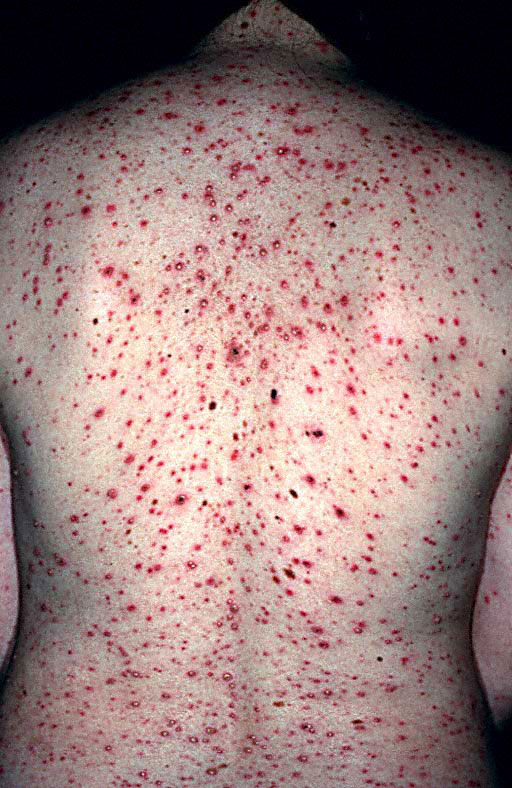
\includegraphics[width=1.2in]{../Imagenes/U.Iowa/Varicela/chicken_pox_picture_01.jpg} &
		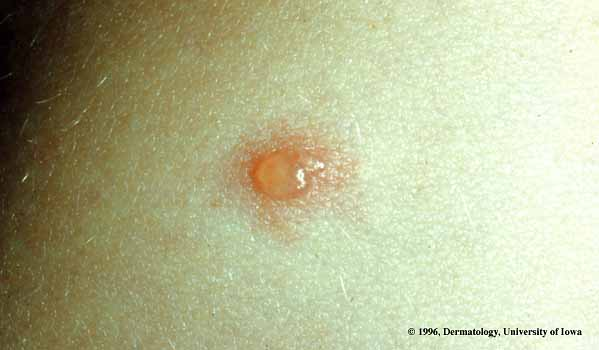
\includegraphics[width=2in]  {../Imagenes/U.Iowa/Varicela/Varicel-02.jpg}
	\end{tabular}
\end{frame}

\begin{frame}
	\frametitle{Elementos que afectan la imagen}
	Problemas
	\begin{itemize}
		\item Ruido \pause
		\item Imperfecciones de la piel \pause
		\item Luces y sombras \pause
		\item Elementos ajenos
	\end{itemize}
\end{frame}

\subsection{T�cnicas utilizadas y medidas adoptadas}
\begin{frame} 
	\frametitle{T�cnicas utilizadas y medidas adoptadas}
	T�cnicas y medidas adoptadas
	\begin{itemize}
		\item Elecci�n de un subconjunto de las im�genes \pause
		\item Ecualizaci�n del histograma (Contrast-limited adaptive histogram equalization) \pause
		\item Reducci�n del ruido o suavizaci�n utilizando un filtro gaussiano \pause
		\item Elecci�n del espacio de color 
	\end{itemize}
\end{frame}

\begin{frame}
	\frametitle{Algunas de las im�genes con las que trabajamos}
	\begin{tabular}{ cc }
		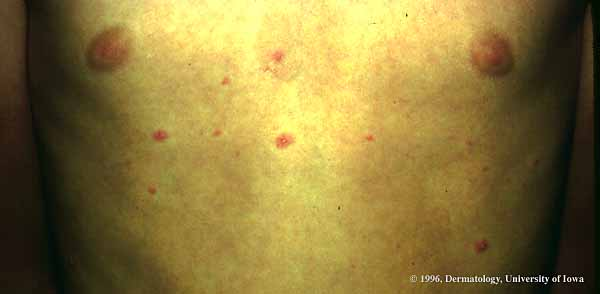
\includegraphics[width=1.6in]{../Imagenes/U.Iowa/Varicela/Varicel-01.jpg} & 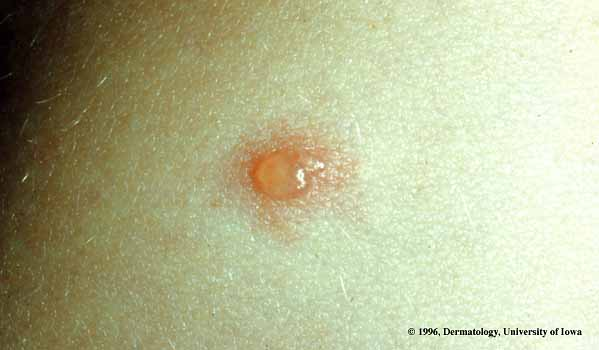
\includegraphics[width=1.6in]{../Imagenes/U.Iowa/Varicela/Varicel-02.jpg} \\
		\includegraphics[width=1.6in]{../Imagenes/U.Iowa/Varicela/Varicel-03.jpg} & \includegraphics[width=1.6in]{../Imagenes/U.Iowa/Varicela/Varicel-04.jpg} \\
	\end{tabular}
\end{frame}

\begin{frame}
	\frametitle{Algunas de las im�genes con las que trabajamos}
	\begin{tabular}{ cc }
		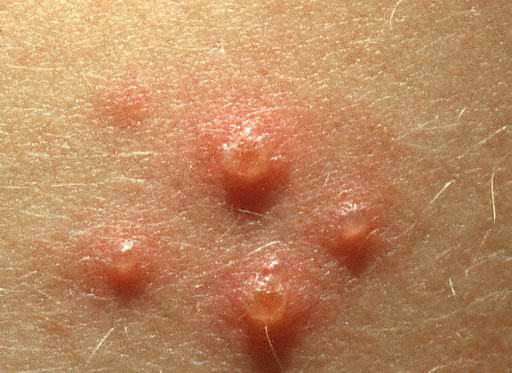
\includegraphics[width=1.6in]{../Imagenes/U.Iowa/Varicela/chicken_pox_primary_lesions_03.jpg} & 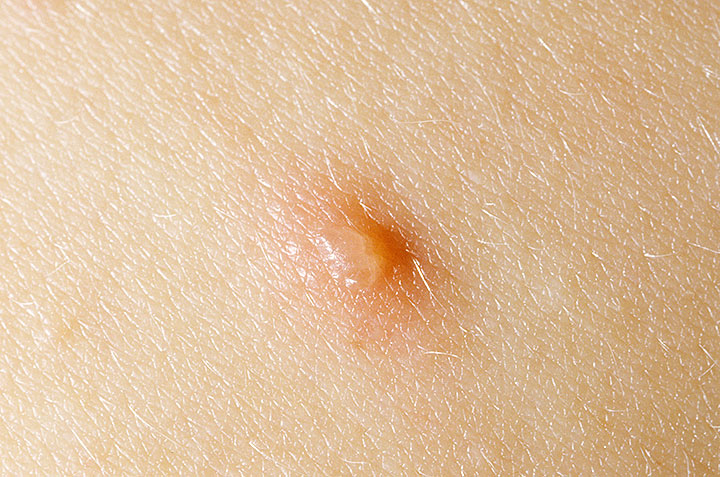
\includegraphics[width=1.6in]{../Imagenes/U.Iowa/Varicela/varicella_20.jpg} \\
	\end{tabular}
\end{frame}
\section{Detecci�n de ves�culas}

\subsection{Espacio de color}
\begin{frame}
	\frametitle{Espacio de color}
	�C�mo representamos los colores y la luz en el ordenador?
	\begin{itemize}
		\item Espacios de color posibles
		\item Luminancia vs Crominancia
		\item YUV vs L*a*b
	\end{itemize}
	Luminancia: detecci�n de bordes\\
	Crominancia: detecci�n de piel y falsos positivos
\end{frame}

\begin{frame}
	\frametitle{Luminancia vs Crominancia}
	\begin{tabular}{cc}
		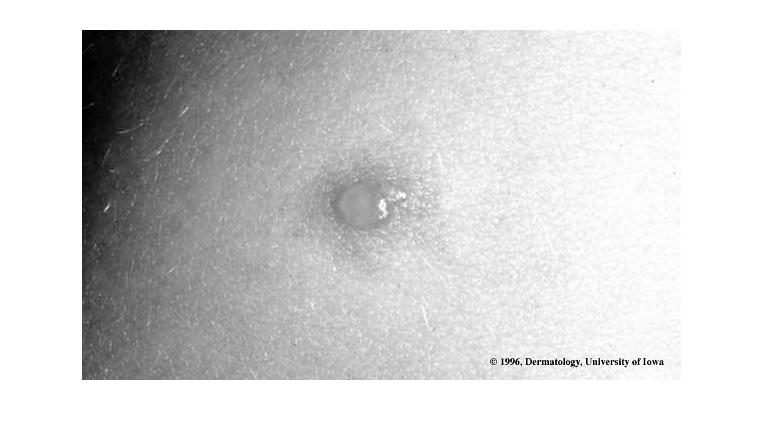
\includegraphics[width=2in]{Resources/CompL-Varicel-02.jpg} & Luminancia - componente L \\
	\end{tabular}
\end{frame}

\begin{frame}
	\frametitle{Luminancia vs Crominancia}
	\begin{tabular}{cc}
		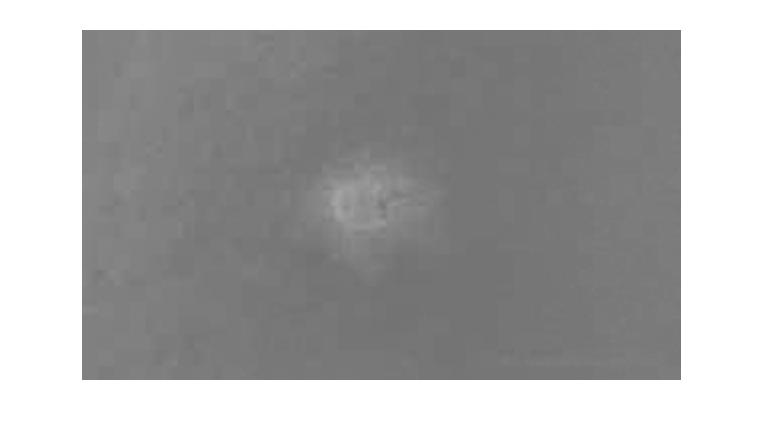
\includegraphics[width=2in]{Resources/CompA-Varicel-02.jpg} & Crominancia - componente a \\
	\end{tabular}
\end{frame}

\begin{frame}
	\frametitle{Luminancia vs Crominancia}
	\begin{tabular}{cc}
		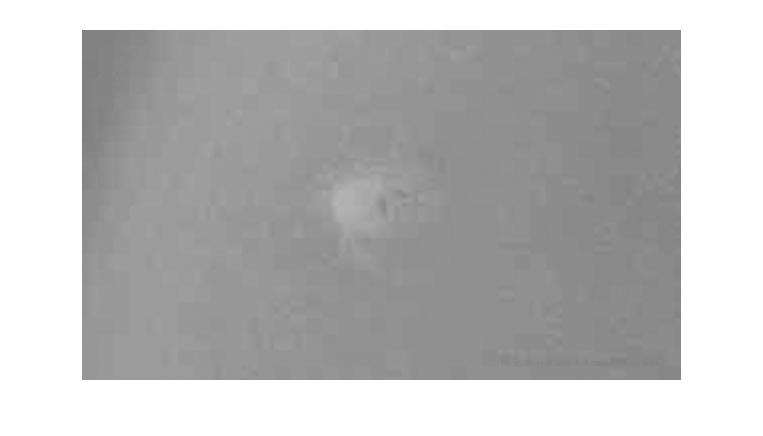
\includegraphics[width=2in]{Resources/CompB-Varicel-02.jpg} & Crominancia - componente b \\
	\end{tabular}
\end{frame}

\subsection{Detecci�n de bordes}
\begin{frame}
	\frametitle{Detecci�n de bordes}
	\begin{itemize}
		\item Resulta sencillo para el ser humano
		\item Borde: frontera entre el objeto y el fondo
		\item Existen varios m�todos (Canny, Roberts, Sobel o Prewitt)
		\item Objetivos de un detector de borde:
		\begin{itemize}
			\item Baja tasa de error
			\item Buena localizaci�n del borde
		\end{itemize}
	\end{itemize}
\end{frame}

\begin{frame}
	\frametitle{M�todo de Canny}
	\begin{itemize}
		\item Robusto contra el ruido
		\item Gran adaptabilidad
		\item Etapas del m�todo:
		\begin{itemize}
			\item Suavizado de la imagen: Filtro gaussiano\\
			\item Obtenci�n del gradiente: Filtro pasa altos en direcci�n vertical y horizontal \\
			\item Supresi�n de puntos que no son m�ximos locales: Adelgazamiento del ancho de los bordes hasta lograr bordes de un p�xel de ancho\\
			\item Umbral con hist�resis: Funci�n de hist�resis basada en dos umbrales; con este proceso se trata de reducir la posibilidad de aparici�n de contornos falsos.\\
		\end{itemize}
	\end{itemize}
\end{frame}

\begin{frame}
	\frametitle{Operaciones morfol�gicas}
	\begin{itemize}
		\item Herramientas muy utilizadas en el procesamiento de im�genes
		\item Simplificar los datos de una imagen
		\item Preservar las caracter�sticas esenciales
		\item Eliminar aspectos irrelevantes
		\item bridge: Une pixeles que est�n separados
		\item Otras operaciones: open, close, clean
	\end{itemize}
\end{frame}

\begin{frame}
	\frametitle{Ejemplo: Bordes detectados en algunas im�genes}
	\begin{columns}[c]
	\column{1.5in}
		\includegraphics[scale=2.33]{Resources/Varicel-03.jpg} \\
		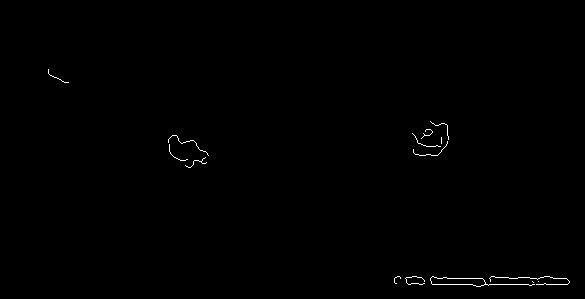
\includegraphics[scale=0.21]{Resources/Varicel-03_bordes_detectados.png} \\
		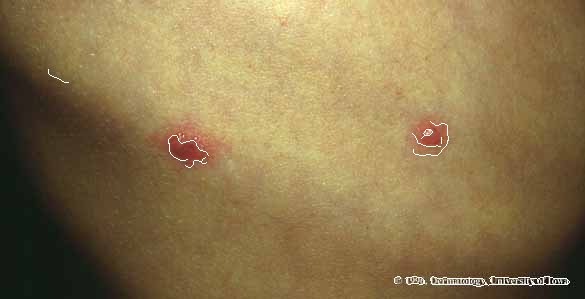
\includegraphics[scale=0.21]{Resources/Varicel-03_imagen_con_bordes.png} \\
	\column{1.5in}	
		\includegraphics[scale=2.8]{Resources/Varicel-04.jpg} \\
		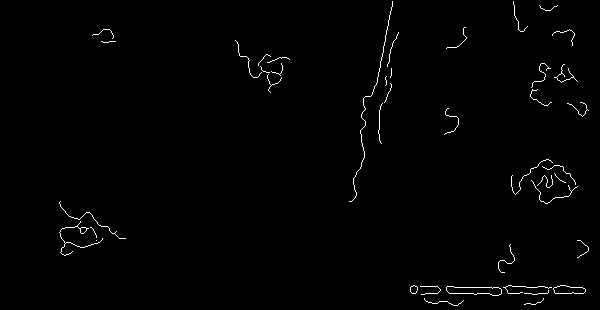
\includegraphics[scale=0.2]{Resources/Varicel-04_bordes_detectados.png} \\
		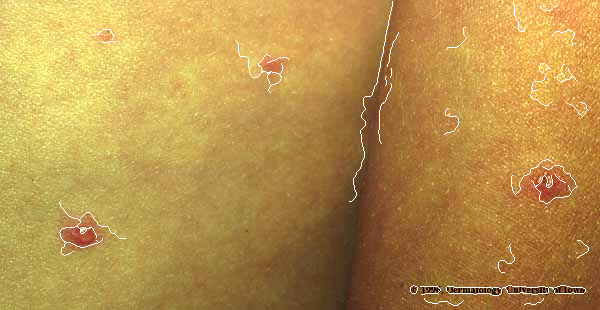
\includegraphics[scale=0.2]{Resources/Varicel-04_imagen_con_bordes.png} \\
	\end{columns}	
\end{frame}

\begin{frame}
	\frametitle{Ejemplo: Bordes detectados en la imagen}
	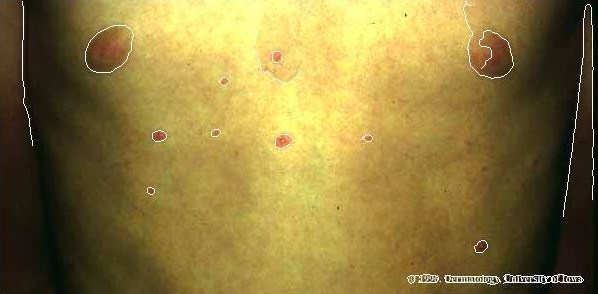
\includegraphics[width=4.3in]{Resources/bordesEnLaImagen-Varicel-01.jpg} \\
\end{frame}

\begin{frame}
	\frametitle{Ejemplo: Bordes detectados}
	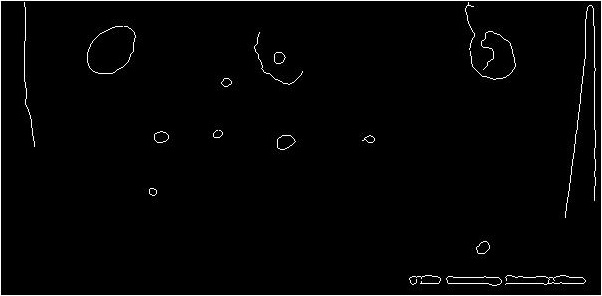
\includegraphics[width=4.3in]{Resources/bordes-Varicel-01.jpg}
\end{frame}

\subsection{Detecci�n de c�rculos}
\begin{frame}
	\frametitle{Detecci�n de c�rculos}
	\begin{itemize}
		\item �Dados los bordes, cu�ndo conforman un c�rculo?
		\item CHT: Circular Hough Transform
		\begin{itemize}
			\item Espacio de Hough
			\item Arreglo de acumulaci�n
		\end{itemize}
		\item Selecci�n de candidatos
		\begin{itemize}
			\item Ponderaci�n con respecto al m�ximo
			\item Umbralizaci�n
		\end{itemize}
	\end{itemize}
\end{frame}

\begin{frame}
	\frametitle{Ejemplo: Imagen con bordes detectados}
	\begin{figure}[h]
		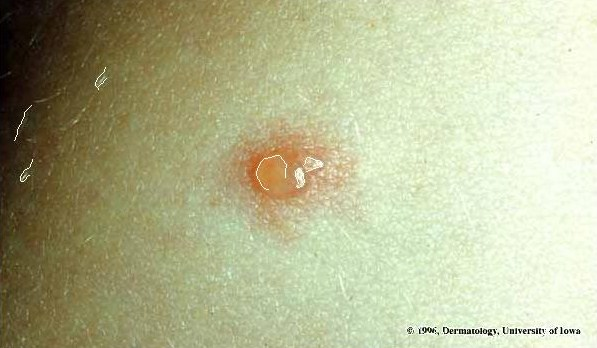
\includegraphics[width=4in]{Resources/resultado-Varicel-02-radio24-bordes.jpg}
	\end{figure}
\end{frame}

\begin{frame}
	\frametitle{Ejemplo: Arreglo de acumulaci�n}
	\begin{figure}[h]
		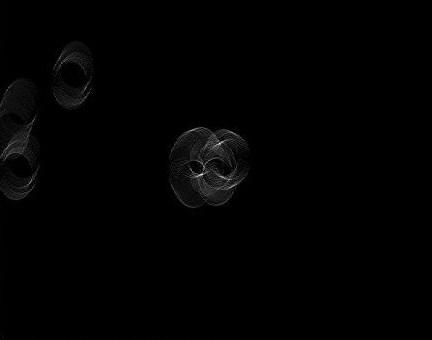
\includegraphics[width=3.5in]{Resources/acumulador-Varicel-02.jpg}
	\end{figure}
\end{frame}

\begin{frame}
	\frametitle{Ejemplo: Imagen con el c�rculo detectado}
	\begin{figure}[h]
		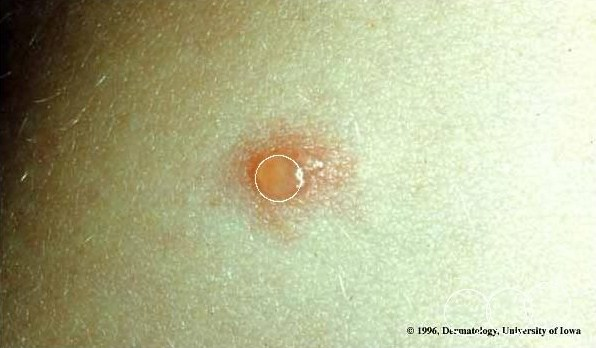
\includegraphics[width=4in]{Resources/resultado-Varicel-02-radio23_1.jpg}
	\end{figure}
\end{frame}

\subsection{Falsos positivos y falsos negativos}
\begin{frame}
	\frametitle{Falsos positivos y falsos negativos}
	\begin{itemize}
		\item Detecci�n de c�rculos redundantes
		\begin{figure}[h]
			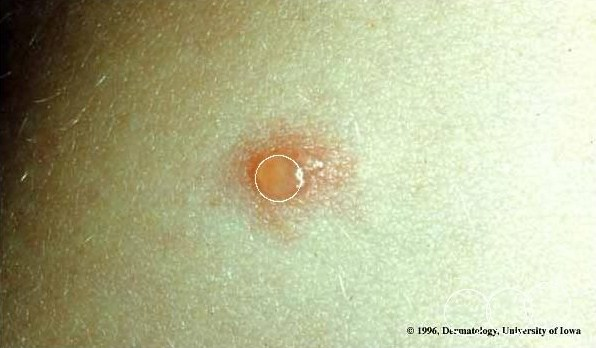
\includegraphics[width=2.2in]{Resources/resultado-Varicel-02-radio23_1.jpg}
			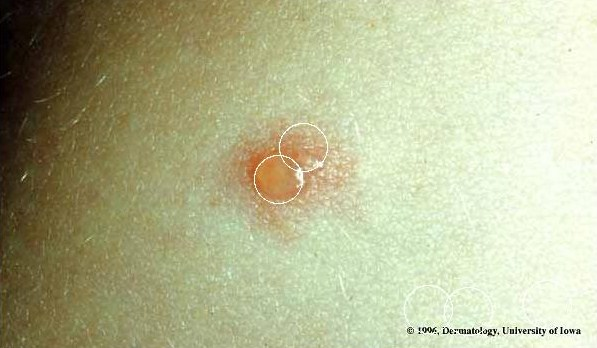
\includegraphics[width=2.2in]{Resources/resultado-Varicel-02-radio24.jpg}
		\end{figure}
		\item An�lisis del interior de la ampolla: Discriminaci�n
	\end{itemize}
\end{frame}

\section{Discriminaci�n entre varicela y otras enfermedades}

\begin{frame}
	\frametitle{Discriminaci�n}
	�Existen diferencias entre la piel sana y las ves�culas? \\
	�Se puede detectar un falso positivo? \\
	�Existen diferencias entre las ves�culas de la varicela y las de otra enfermedad? \\
	�Se pueden desarrollar t�cnicas de detecci�n y discriminaci�n autom�ticas? \\
	\begin{itemize}
		\item An�lisis comparativo entre la varicela y la piel sana \\
		\item An�lisis comparativo entre la varicela y otra enfermedad \\
	\end{itemize}
\end{frame}

\begin{frame}
	\frametitle{T�cnicas utilizadas}
	\begin{itemize}

		\item T�cnicas basadas en el histograma de color
		\begin{itemize}
			\item Construcci�n de un histograma de referencia
			\item An�lisis de casos muestra: comparaciones entre el histograma de cada ves�cula y
			\begin{itemize}
				\item el histograma promedio de varicela
				\item el histograma promedio de herpes z�ster
			\end{itemize}
		\end{itemize}

		\item T�cnicas basadas en la comparaci�n de media poblacional
		\begin{itemize}
			\item Comparaci�n por distancia de Mahalanobis
			\item Test de distribuci�n Hotelling T-Cuadrada
			\item Test de ANOVA
		\end{itemize}
		
	\end{itemize}
\end{frame}

\subsection{Construcci�n de un histograma de referencia}
\begin{frame}
	\frametitle{Histogramas sobre espacios de color}
	An�lisis del histograma de las distintas componentes de color \\
	\begin{itemize}
		\item De forma individual \\
		\item Histograma bivariado de a pares de componentes \\
	\end{itemize}
	�Qu� espacio de color utilizar? \\
	\begin{itemize}
		\item L*a*b: Dos componentes de crominancia \\
		\item RGB: Informaci�n sobre el corrimiento al rojo de las ves�culas en relaci�n a la piel normal \\
	\end{itemize}
	\pause
	\textbf{Histogramas de referencia: Valores extra�dos de un conjunto de ves�culas conocidas, contra los cuales comparar las nuevas ves�culas}
\end{frame}

\begin{frame}
	\frametitle{Histogramas}
	\begin{figure}[h!]
	\centering
	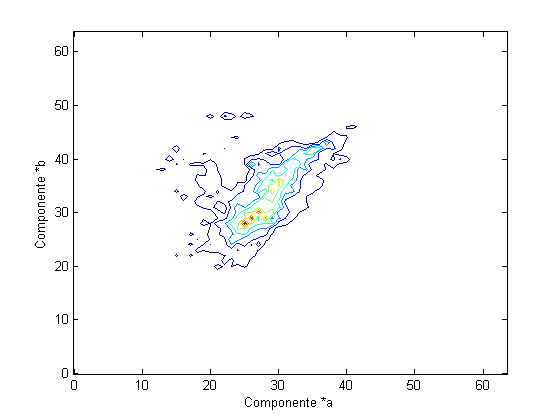
\includegraphics[scale=0.25]{Resources/histograma-promedio-varicela-ab.png}
	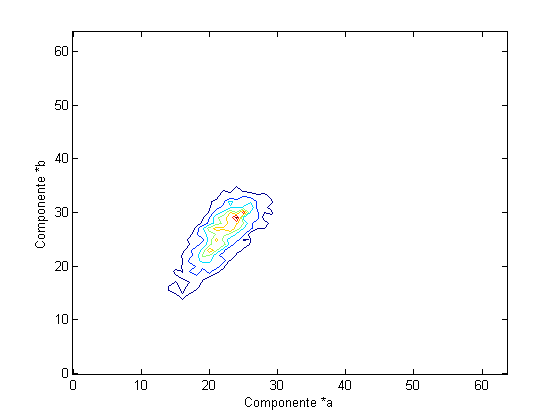
\includegraphics[scale=0.25]{Resources/histograma-promedio-herpes-ab.png}
	\caption{Histogramas bivariados promedio de varicela y herpes z�ster, sobre las variables de crominancia *a y *b. \textbf{Izq:} Varicela. \textbf{Der:} Herpes z�ster. \label{fig:histogramasPromedio}}
	\end{figure}
\end{frame}

\begin{frame}
	\frametitle{Histogramas}
	\begin{itemize}
		\item Leve corrimiento hacia el rojo del histograma de varicela \\
		\item Dispersi�n de valores mayor en el histograma del espacio RGB \\
		\item Mayor concentraci�n de valores para el espacio de color L*a*b \\
	\end{itemize}

	\begin{figure}[h!]
	\centering
	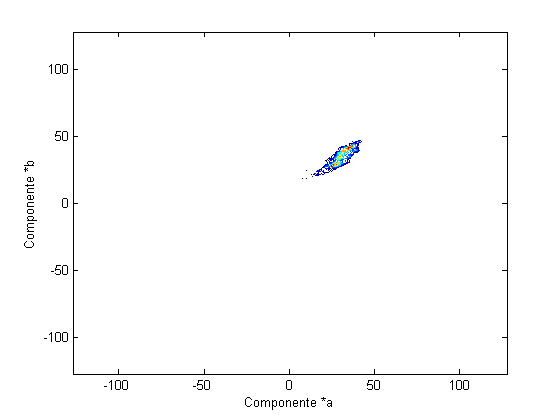
\includegraphics[scale=0.15]{Resources/contourAB-ch03.png}
	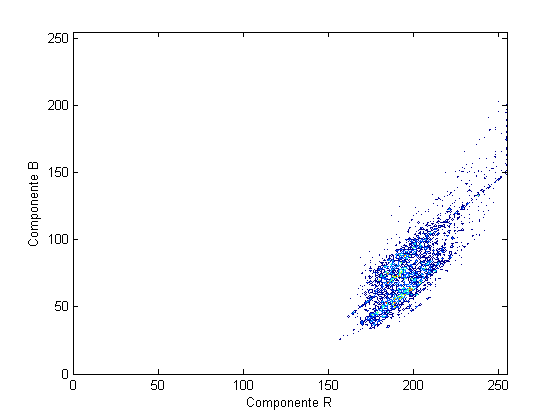
\includegraphics[scale=0.15]{Resources/contourRB-ch03.png}
	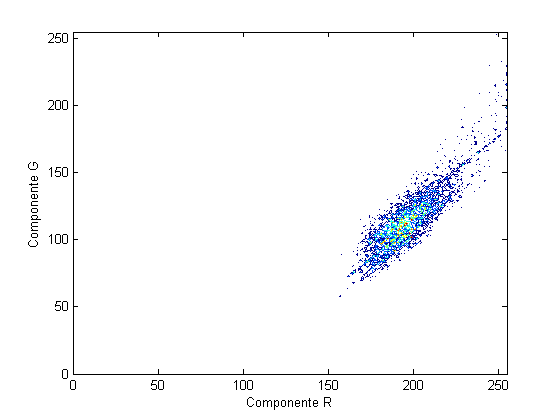
\includegraphics[scale=0.15]{Resources/contourRG-ch03.png}
	\caption{Histogramas bivariados promedio de la imagen izquierda de la figura, \textbf{Arriba izq:} , Variables de crominancia *a y *b. \textbf{Arriba der:} Variables de crominancia R y B. \textbf{Abajo:} Variables de crominancia R y B. \label{fig:histogramasPromedioch03}}
	\end{figure}
\end{frame}

\subsection{Comparaci�n entre una ves�cula y la piel normal}
\begin{frame}
	\frametitle{Divergencia entre histogramas}
	Mediciones de distancia (o divergencia) entre histogramas. \\
	\textbf{Indicador buscado:} Si la distancia del histograma de la ves�cula candidata al promedio est� por debajo o por encima de cierto umbral. \\
	Evaluaci�n sobre: \\
	\begin{itemize}

		\item Norma 1
		\item Norma 2
		\item Divergencia de Kullback-Leibler (KLD)

	\end{itemize}
\end{frame}

\begin{frame}
	\frametitle{Divergencia de Kullback-Leibler}
	Mide la diferencia entre dos distribuciones P y Q. \\
	\begin{itemize}

		\item P representa la distribuci�n real de datos u observaciones (en este caso, la ves�cula observada)
		\item Q representa el modelo te�rico (en este caso, el histograma promedio)

	\end{itemize}
	Mide la cantidad esperada de bits extra requeridos para codificar ejemplos de P utilizando un c�digo basado en Q. \\
	Tambi�n llamada ``entrop�a relativa''. \\
\end{frame}

\begin{frame}
	\frametitle{Divergencia de Kullback-Leibler}
	\[
	KLD(P||Q) = \displaystyle\sum_{i} P(i) \ln(\frac{P(i)}{Q(i)}).
	\]

	La KLD no es una distancia, porque no cumple con la condici�n de simetr�a. \\
	Utilizamos una variante sim�trica de la KLD: \\

	\[
	KLD_{sym}(P||Q) = \frac{KLD(P||Q) + KLD(Q||P)}{2}.
	\]

\end{frame}

\begin{frame}
	\frametitle{Algunas im�genes analizadas}
\tiny
\begin{figure}[ht]
\centering
	\begin{columns}[c]
	\column{1.2in}
		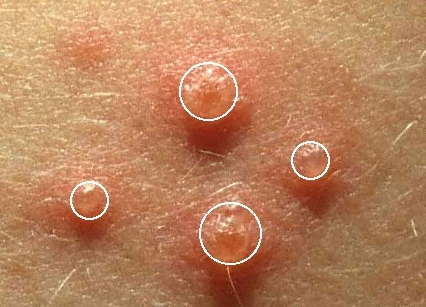
\includegraphics[width=1in]{Resources/chicken_pox_primary_lesions_03_concirculos_crop.jpg} (a) \\
		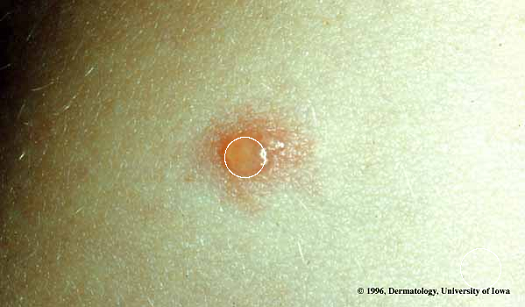
\includegraphics[width=1in]{Resources/Varicel-02_resultado_con_ecualizacion_crop.png} (b) \\
	\column{1.2in}	
		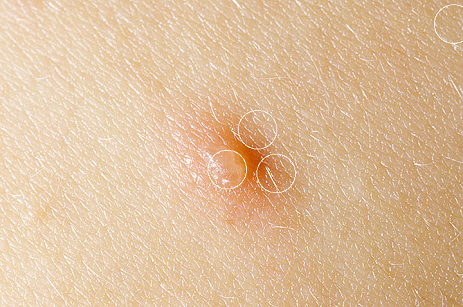
\includegraphics[width=1in]{Resources/Varicella_20_resultado_con_ecualizacion_crop.png} (c) \\
		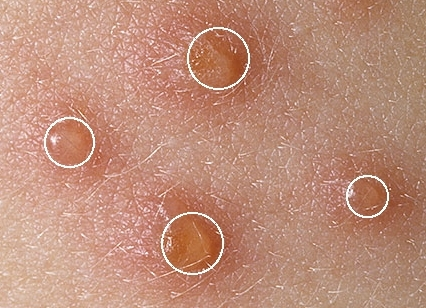
\includegraphics[width=1in]{Resources/varicella_34_concirculos_crop.jpg} (d) \\
	\column{1.2in}	
		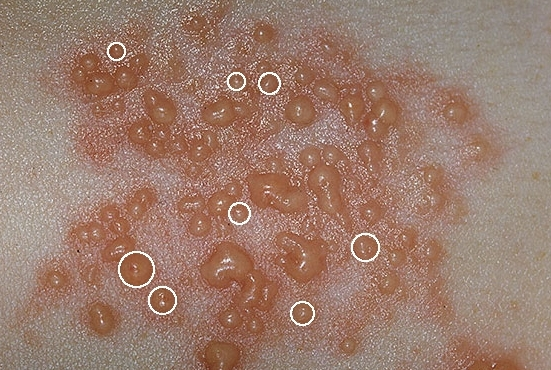
\includegraphics[width=1in]{Resources/herpes_zoster_114_concirculos_crop.jpg} (e) \\
		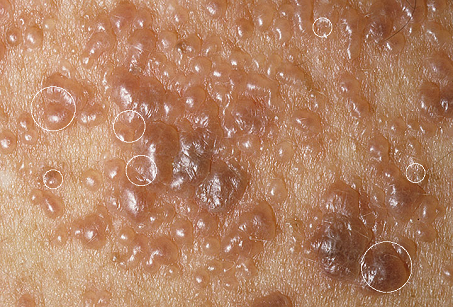
\includegraphics[width=1in]{Resources/herpes_zoster_309_concirculos_crop.png} (f) \\
		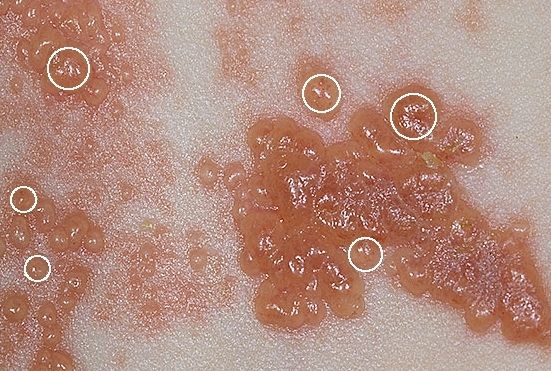
\includegraphics[width=1in]{Resources/herpes_zoster_8_concirculos_crop.jpg} (g) \\
	\end{columns}	
	\normalsize
	\caption{Ves�culas analizadas. (a) - (b) - (c) - (d) Ves�culas de varicela. (e) - (f) - (g) Ves�culas de herpes z�ster.\label{fig:imagenesKLD}}
\end{figure}

\end{frame}


\begin{frame}
	\frametitle{Resultados: Comparaci�n entre varicela y piel}
	Los mejores resultados se observan sobre $KLD_{A}$, $KLD_{B}$ y $KLD_{AB}$. \\
\tiny
	\begin{table}[ht]
	\centering
	\begin{tabular}[pos]{ l | l | c | c | c }
		Imagen & C�rculo detectado & $KLD_{A}$ & $KLD_{B}$ & $KLD_{AB}$ \\
	\hline
	Varicela 1 & Falso positivo	& $24.26$	& $16.98$	& $32.60$ \\
	Varicela 2 & Falso positivo	& $27.54$	& $17.22$	& $45.41$ \\
	Varicela 3 & Falso positivo	& $25.71$	& $17.39$	& $28.28$ \\
	Varicela 4 & Falso positivo	& $22.52$	& $15.74$	& $24.90$ \\
	\hline
	Varicela 1 & Ves�cula 1	& $0.33$	& $1.69$	& $ 6.43$     \\
	Varicela 1 & Ves�cula 2	& $0.51$	& $1.16$	& $ 7.15$     \\
	Varicela 1 & Ves�cula 3	& $1.13$	& $4.46$	& $11.39$     \\
	Varicela 1 & Ves�cula 4	& $0.68$	& $2.60$	& $11.17$     \\
	Varicela 2 & Ves�cula 1	& $2.00$	& $0.35$	& $12.87$     \\
	Varicela 3 & Ves�cula 1	& $2.17$	& $3.87$	& $12.66$     \\
	Varicela 3 & Ves�cula 2	& $0.68$	& $0.50$	& $ 6.06$     \\
	Varicela 3 & Ves�cula 3	& $1.49$	& $0.49$	& $ 7.01$     \\
	Varicela 3 & Ves�cula 1	& $1.83$	& $5.07$	& $11.46$     \\
	\end{tabular}
	\caption{Mediciones de KLD entre histogramas de c�rculos detectados y los histogramas promedio, sobre componentes *a y *b. \label{tab:KLD}}
	\end{table}
\normalsize

\end{frame}


\subsection{Comparaci�n entre ves�culas de varicela y herpes z�ster}
\begin{frame}
	\frametitle{Comparaci�n entre ves�culas de varicela y herpes z�ster}
	Mediciones realizadas sobre:
	\begin{itemize}

		\item Un conjunto de c�rculos detectados de varicela
		\item Un conjunto de c�rculos detectados de herpes z�ster
		\item Comparaci�n contra el histograma promedio de la varicela
	\end{itemize}
	
	Resultado esperado:
	
	\begin{itemize}

		\item Divergencias de las ves�culas de varicela: dentro un intervalo observable
		\item Divergencias de los histogramas de herpes: pocas o ninguna de las ves�culas dentro de ese intervalo

	\end{itemize}

\end{frame}


\begin{frame}
	\frametitle{Resultados: Comparaci�n entre varicela y herpes z�ster}

	Resultados no alentadores: \\

	\tiny
\begin{table}[ht]
\centering
\begin{tabular}[pos]{ l | l | c | c | c }
	Imagen \ref{fig:imagenesKLD}  & C�rculo detectado & $KLD_{A}$ & $KLD_{B}$ & $KLD_{AB}$ \\
\hline
Herpes 1 & Ves�cula 1	&  $ 7.86$	&	$10.42$	&	$18.73$	\\
Herpes 1 & Ves�cula 2	&  $17.79$	&	$15.80$	&	$22.70$	\\
Herpes 1 & Ves�cula 3	&  $ 7.24$	&	$11.72$	&	$20.27$	\\
Herpes 1 & Ves�cula 4	&  $ 8.39$	&	$14.63$	&	$20.15$	\\
Herpes 1 & Ves�cula 5	&  $ 7.42$	&	$10.35$	&	$17.85$	\\
Herpes 1 & Ves�cula 6	&  $ 5.41$	&	$ 4.95$	&	$15.72$	\\

Herpes 2 & Ves�cula 1	&	$4.03$	&	$5.78$	&	$12.86$ 	\\
Herpes 2 & Ves�cula 2	&	$2.93$	&	$1.99$	&	$11.70$ 	\\
Herpes 2 & Ves�cula 3	&	$6.35$	&	$6.79$	&	$15.60$	\\

Herpes 3 & Ves�cula 1	&	$26.25$	&	$24.90$	&	$31.63$	\\
Herpes 3 & Ves�cula 2	&	$ 4.81$	&	$ 9.57$	&	$19.64$	\\
\hline
Varicela 1 & Ves�cula 1	& $0.33$	& $1.69$	& $ 6.43$      \\
Varicela 1 & Ves�cula 2	& $0.51$	& $1.16$	& $ 7.15$      \\
Varicela 1 & Ves�cula 3	& $1.13$	& $4.46$	& $11.39$      \\
Varicela 1 & Ves�cula 4	& $0.68$	& $2.60$	& $11.17$      \\
Varicela 2 & Ves�cula 1	& $2.00$	& $0.35$	& $12.87$      \\
Varicela 3 & Ves�cula 1	& $2.17$	& $3.87$	& $12.66$      \\
Varicela 3 & Ves�cula 2	& $0.68$	& $0.50$	& $ 6.06$      \\
Varicela 3 & Ves�cula 3	& $1.49$	& $0.49$	& $ 7.01$      \\
Varicela 3 & Ves�cula 1	& $1.83$	& $5.07$	& $11.46$      \\
\end{tabular}
\caption{Mediciones de KLD entre c�rculos detectados de varicela y herpes z�ster, contra el histograma promedio de varicela \label{tab:KLDvh}}
\end{table}
\normalsize

\end{frame}



\begin{frame}

	\frametitle{Pruebas adicionales}

	\begin{itemize}

		\item Medici�n de distancias: la norma 1 y norma 2
		\item Histogramas de componentes individuales de RGB
		\item Histogramas bivariados de componentes de RGB
		\item Histogramas de componentes individuales de L*a*b

	\end{itemize}
	
	En ninguna de estas pruebas se observ� que el conjunto de mediciones de la varicela y del herpes z�ster cayeran en intervalos disjuntos.
	
\end{frame}


\begin{frame}

	\frametitle{Conclusi�n parcial}

	
	\begin{itemize}

		\item Para este conjunto de im�genes utilizadas, el an�lisis de la divergencia de histogramas entre la varicela y el herpes z�ster no alcanza para determinar un umbral para distinguir entre ambas enfermedades. \\
		\item El mismo m�todo arroja resultados favorables para determinar si una ves�cula detectada es un falso positivo (piel) o una ves�cula real de varicela.

	\end{itemize}
	
\end{frame}




\subsection{T�cnicas basadas en la comparaci�n de media poblacional}
\begin{frame}
	\frametitle{Distancia de Mahalanobis}
	La distancia Mahalanobis entre dos vectores aleatorios multidimensionales $x$ e $y$, provenientes de la misma poblaci�n, se define como: \\

\begin{equation}
d_{mahal}(\vec{x},\vec{y}) = \sqrt{(\vec{x}-\vec{y})^{T} S^{-1} (\vec{x}-\vec{y})}.
\end{equation}

Siendo $\vec{x}$ e $\vec{y}$ los vectores entre los cu�les se desea medir la distancia.

\end{frame}


\begin{frame}
	\frametitle{Distancia de Mahalanobis}

	La distancia Mahalanobis entre un vector multivariado $x$ a un conjunto de valores con media $\mu$, y matriz de covarianza $S$, se define como: \\

\begin{eqnarray}
D_{mahal}(x) & = & \sqrt{(x-\mu)^{T} S^{-1} (x-\mu)}.
\end{eqnarray}

\begin{eqnarray}
x & = & (x_{1},x_{2},x_{3},...,x_{n})^{T} \nonumber \\
\mu & = & (\mu_{1},\mu_{2},\mu_{3},...,\mu_{n})^{T} \nonumber
\end{eqnarray}

\end{frame}

\begin{frame}
	\frametitle{Distancia de Mahalanobis}

	\begin{itemize}
		\item Similar a la distancia eucl�dea
		\item Sirve para determinar la similitud entre los dos vectores
		\item A diferencia de la distancia eucl�dea, tiene en cuenta la correlaci�n entre las variables
		\item Se adapta mejor para distribuciones sim�tricas no esf�ricas
		\item Es �til para determinar la distancia de un punto a la media de una distribuci�n, o la distancia entre las medias de dos distribuciones
		\item Entonces, puede indicar si los p�xeles de una ves�cula detectada son m�s similares a los de varicela o a los de herpes z�ster
	\end{itemize}
	
\end{frame}


\begin{frame}
	\frametitle{Resultados: Comparaci�n por distancia de Mahalanobis}
	
	Resultados favorables para discriminar los falsos positivos, pero no para distinguir entre ves�culas de varicela y de herpes z�ster. \\
	
	\tiny
\begin{table}[h!]
\centering

\begin{tabular}[pos]{ l | l | c | c | c | c | c | c }
Imagen \ref{fig:imagenesKLD} & C�rculo detectado & $D_{L}$ & $D_{A}$ & $D_{B}$ & $D_{LA}$ & $D_{LB}$ & $D_{AB}$ \\
\hline
Varicela 1 & Falso positivo 1	&	$13.2$	&	$19.2$	&	$0.1$	&	$20.5$	&	$23.4$	&	$35.4$	\\
Varicela 1 & Falso positivo 2	&	$ 9.5$	&	$19.4$	&	$0.0$	&	$20.0$	&	$16.1$	&	$34.2$	\\
Varicela 1 & Falso positivo 3	&	$ 5.1$	&	$14.6$	&	$0.0$	&	$15.5$	&	$ 8.0$	&	$24.6$	\\
Varicela 1 & Falso positivo 4	&	$11.0$	&	$15.3$	&	$0.1$	&	$16.7$	&	$19.2$	&	$27.7$	\\
\hline
Varicela 1 & Ves�cula 1	&	$1.5$	&	$3.0$	&	$0.9$	&	$ 5.3$	&	$3.0$	&	$3.7$	\\
Varicela 1 & Ves�cula 2	&	$3.6$	&	$4.5$	&	$1.2$	&	$11.7$	&	$7.5$	&	$5.3$	\\
Varicela 1 & Ves�cula 3	&	$1.7$	&	$1.6$	&	$0.3$	&	$ 3.5$	&	$2.4$	&	$2.0$	\\
Varicela 1 & Ves�cula 4	&	$2.5$	&	$4.7$	&	$0.9$	&	$ 7.5$	&	$4.1$	&	$5.6$	\\
\hline
Herpes 1 & Ves�cula 1 & $0.90$	&	$2.70$	&	$1.60$	&	$ 6.29$	&	$4.19$	&	$3.70$	\\
Herpes 1 & Ves�cula 2 & $1.14$	&	$2.64$	&	$1.16$	&	$ 3.48$	&	$1.97$	&	$3.50$	\\
Herpes 2 & Ves�cula 1 & $2.94$	&	$2.69$	&	$1.00$	&	$13.53$	&	$8.38$	&	$3.15$	\\
Herpes 2 & Ves�cula 2 & $1.74$	&	$4.75$	&	$1.63$	&	$14.37$	&	$7.21$	&	$5.38$	\\
Herpes 3 & Ves�cula 1 & $1.39$	&	$6.83$	&	$1.95$	&	$17.51$	&	$6.48$	&	$7.53$	\\
Herpes 3 & Ves�cula 2 & $0.98$	&	$3.62$	&	$1.86$	&	$ 7.59$	&	$4.42$	&	$4.02$	\\

\end{tabular}
\caption{Mediciones de promedio de $D_{mahal}$ entre c�rculos detectados de varicela, herpes z�ster y falsos positivos, contra el histograma promedio de varicela \label{tab:Mahal}}
\end{table}
\normalsize

\end{frame}



\begin{frame}
	\frametitle{Distribuci�n poblacional del color de la ves�culas}

	\begin{itemize}
		\item Distribuciones de color de ambas enfermedades muy similares
		\item �Pertenecen a una misma poblaci�n?
		\item �Son muestras de la misma variable aleatoria?
		\item Pruebas estad�sticas para determinar su homogeneidad
		\begin{itemize}
			\item Test de distribuci�n Hotelling T-Cuadrada
			\item Test de ANOVA
		\end{itemize}
	\end{itemize}

\end{frame}


\begin{frame}
	\frametitle{Test de distribuci�n Hotelling T-Cuadrada}

	\begin{itemize}
		\item Asumiendo dos distribuciones multinormales y con matrices de covarianza id�nticas, \\
		dada la hip�tesis nula $H_{0}$ que ambas medias son iguales $\mu_{1} = \mu_{2}$, \\
		puede indicar si hay suficiente evidencia para rechazar $H_{0}$. \\
		
		\item Vector de diferencia utilizado: distancia de Mahalanobis.

		\begin{itemize}
			\item Entre los p�xeles de una ves�cula de varicela y el histograma promedio de varicela
			\item Entre los p�xeles de una ves�cula de herpes z�ster y el histograma promedio de varicela
		\end{itemize}
	\end{itemize}
\end{frame}


\begin{frame}
	\frametitle{Resultados: Test de distribuci�n Hotelling T-Cuadrada}

	\begin{itemize}
		\item En todos los casos el test arroj� $p = 0$
		\item Indica que, utilizando este test, \textbf{no hay evidencia suficiente} para rechazar la hip�tesis nula de que ambas distribuciones tienen la misma media.
	\end{itemize}
\end{frame}

\begin{frame}
	\frametitle{Test de ANOVA (Analysis of Variance)}

	Evaluar si se puede rechazar la hipotesis nula $H_{0}$ de igualdad de las medias. \\
	\begin{itemize}
		\item Tomar im�genes representativas
		\item Contruir una clase con los valores para las ves�culas de cada imagen
		\item Medir la distancia entre las medias de las clases (e intraclases tambi�n)
	\end{itemize}
\tiny
\begin{figure}[h!]
	\centering
	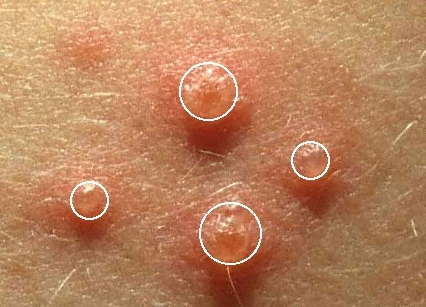
\includegraphics[width=0.8in]{Resources/chicken_pox_primary_lesions_03_concirculos_crop.jpg} (a)\hspace{4pt}
	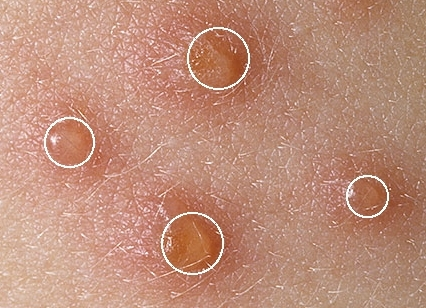
\includegraphics[width=0.8in]{Resources/varicella_34_concirculos_crop.jpg} (b)\hspace{4pt}
	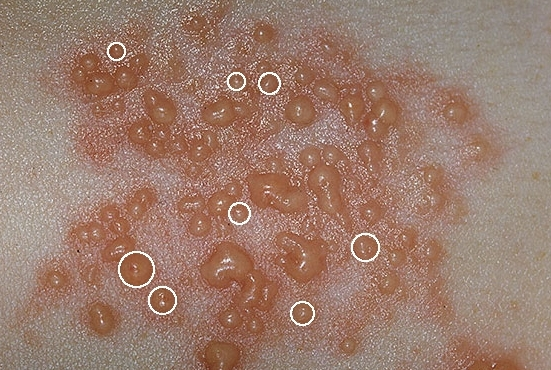
\includegraphics[width=0.8in]{Resources/herpes_zoster_114_concirculos_crop.jpg} (c)\hspace{4pt}
	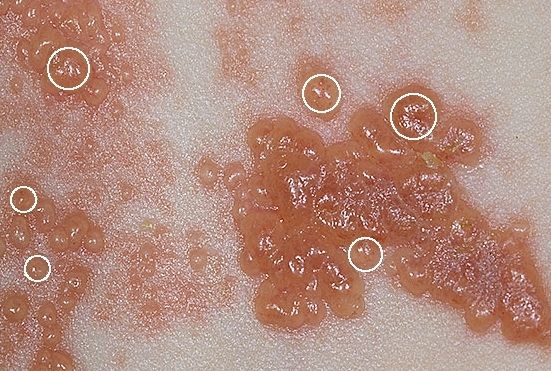
\includegraphics[width=0.8in]{Resources/herpes_zoster_8_concirculos_crop.jpg} (d)
	\caption{Ves�culas detectadas. (a) - (b) Ves�culas de varicela. (c) - (d) Ves�culas de herpes z�ster.\label{fig:imagenesAnova}}
\end{figure}
\normalsize
\end{frame}

\begin{frame}
	\frametitle{Mediciones: Diferencias entre medias de varicela y herpes z�ster (comp. *a)}

	\tiny
\begin{table}[h]
\centering
\begin{tabular}[pos]{ c | c | c }
Distancia entre medias & Intervalo & Comparaci�n de medias \\

\hline
$\mu_{(a)} - \mu_{(c)} = 9.1967$	&	$[ 8.8831  , \ 9.5104  ]$	&	Interclases \\
$\mu_{(a)} - \mu_{(d)} = 6.1135$	&	$[ 5.8445  , \ 6.3826  ]$	&	Interclases  \\
$\mu_{(b)} - \mu_{(c)} = 6.5746$	&	$[ 6.2689  , \ 6.8802  ]$	&	Interclases  \\
$\mu_{(b)} - \mu_{(d)} = 3.4913$	&	$[ 3.2317  , \ 3.7509  ]$	&	Interclases  \\
\hline
$\mu_{(a)} - \mu_{(b)} = 2.6222$	&	$[ 2.3835  , \ 2.8609  ]$	&	Intraclases  \\
$\mu_{(c)} - \mu_{(d)} = -3.0832$	&	$[ -3.4131  , \ -2.7533  ]$	&	Intraclases  \\

\end{tabular}
\caption{Comparaci�n entre clases de varicela y herpes z�ster, sobre componente *a \label{tab:comparacionMediasCompA}}
\end{table}
\normalsize

\end{frame}

\begin{frame}
	\frametitle{Mediciones: Diferencias entre medias de varicela y herpes z�ster (comp. *Cb)}

	\tiny
\begin{table}[h]
\centering
\begin{tabular}[pos]{ c | c | c }
Distancia entre medias & Intervalo & Comparaci�n de medias \\

\hline
$\mu_{(a)}- \mu_{(c)} =  -8.3343  $   &   $[   -8.6310    , \      -8.0376    ]$	&	Interclases \\
$\mu_{(a)}- \mu_{(d)} =   -8.0301 $   &   $[  -8.2846     , \     -7.7756    ]$	&	Interclases \\
$\mu_{(b)}- \mu_{(c)} =  5.2527   $   &   $[   4.9636   , \      5.5418     ]$	&	Interclases \\
$\mu_{(b)}- \mu_{(d)} =   4.9486  $   &   $[ 4.7030       , \     5.1941    ]$	&	Interclases \\
\hline
$\mu_{(a)} - \mu_{(b)} = -3.0816$	&	$[ -3.3073  , \ -2.8558  ]$	&	Intraclases \\
$\mu_{(c)} - \mu_{(d)} = 0.3042$	&	$[ -0.0079  , \ 0.6162  ]$   \textbf{(**)}	&	Intraclases \\

\end{tabular}
\caption{Comparaci�n entre clases de varicela y herpes z�ster, sobre componente *Cb \label{tab:comparacionMediasCompCb}}
\end{table}
\normalsize

\end{frame}

\begin{frame}
	\frametitle{Mediciones: Diferencias entre medias de varicela y herpes z�ster (comp. *Cr)}

	\tiny
\begin{table}[h]
\centering
\begin{tabular}[pos]{ c | c | c }
Distancia entre medias & Intervalo & Comparaci�n de medias \\

\hline
$\mu_{(a)}- \mu_{(c)} = 12.1550   $	&	$[  11.8231    , \      12.4869  ]$	&	Interclases \\
$\mu_{(a)}- \mu_{(d)} =   8.9064  $	&	$[ 8.6217      , \      9.1910    ]$	&	Interclases \\
$\mu_{(b)}- \mu_{(c)} =  -8.0765  $	&	$[   -8.3999     , \     -7.7532    ]$	&	Interclases \\
$\mu_{(b)}- \mu_{(d)} =   -4.8279 $	&	$[ -5.1026      , \    -4.5532    ]$	&	Interclases \\
\hline
$\mu_{(a)} - \mu_{(b)} = 4.0785$	&	$[ 3.8259  , \ 4.3310  ]$	&	Intraclases \\
$\mu_{(c)} - \mu_{(d)} = -3.8426$	&	$[ -3.5977  , \ -2.8996  ]$	&	Intraclases \\

\end{tabular}
\caption{Comparaci�n entre clases de varicela y herpes z�ster, sobre componente *Cr \label{tab:comparacionMediasCompCr}}
\end{table}
\normalsize

\end{frame}


\begin{frame}
	\frametitle{Resultados: Test de ANOVA}

	Asumiendo una distribuci�n normal de los valores y varianzas iguales, \\
	Hip�tesis nula $H_{0}$: las medias de los colores de las ves�culas de varicela y herpes z�ster son iguales.

	\footnotesize
	\begin{itemize}
		\item Componente a*: diferencia $\mu_{\scriptsize\textrm{(varicela)}}- \mu_{\scriptsize\textrm{(herpesz�ster)}} = 5.8608$, \\
		con una confianza del 100\% en el intervalo $[5.7044 \quad 6.0171]$.
		\item Componente *Cb: diferencia $\mu_{\scriptsize\textrm{(varicela)}}- \mu_{\scriptsize\textrm{(herpesz�ster)}} = -6.4700$, \\
		con una confianza del 100\% en el intervalo $[-6.6175 \quad -6.3225]$.
		\item Componente *Cr: diferencia $\mu_{\scriptsize\textrm{(varicela)}}- \mu_{\scriptsize\textrm{(herpesz�ster)}} = 7.9246$, \\
		con una confianza del 100\% en el intervalo $[7.7563 \quad 8.0929]$.
	\end{itemize}
\normalsize

\end{frame}


\begin{frame}
	\frametitle{Resultados: Test de ANOVA}

	\begin{itemize}
		\item Existe suficiente evidencia estad�stica para rechazar la hip�tesis nula de que las medias de las dos clases son iguales
		\item Adem�s, la diferencia interclases es mayor que la diferencia intraclases
		\item Sin embargo, hay demasiada variabilidad en los datos para poder aceptar la otra hip�tesis nula: que las im�genes pertenecientes a la misma clase tienen la misma media.
	\end{itemize}
	
\end{frame}


\section{Conclusiones}

\begin{frame}
	\frametitle{Trabajo futuro}
	\begin{itemize}
		\item Detecci�n de piel
		\item Detecci�n de ampollas que no tengan forma circular
		\item Detecci�n de patrones en las im�genes
		\begin{itemize}
			\item Buscar caracter�sticas que permitan determinar cu�ndo se est� en presencia de la varicela
			\item Aprendizaje autom�tico sobre el histograma del color de las ampollas detectadas
		\end{itemize}
	\end{itemize}
\end{frame}

\begin{frame}
	\frametitle{Preguntas?}
	...
\end{frame}

\begin{frame}
	\frametitle{Gracias!}
	Virginia Arroyo (virginia.arroyo@gmail.com)\\
	Juli�n Oyola (joyola@dc.uba.ar)\\
	Anita Ruedin (ana.ruedin@dc.uba.ar)
\end{frame}

\chapter*{Agradecimientos}

\noindent Queremos dar las gracias a nuestras familias y amigos por el apoyo incondicional.

\begin{thebibliography}{200}

\small

\bibitem{RA01} Ramello, Pedro Mart�n.
``Comparaci�n de m�todos de detecci�n de piel en modelos de color YCbCr y HSI para reconocimiento de caras'', 2005.

\bibitem{LC01} Luis Coll, Dante Chinchilla, Constanza Coll, Fernando Stengel, Horacio Cabo.
``An�lisis digital de im�genes en lesiones pigmentadas de la piel. Diagn�stico precoz del melanoma'', 2007.

\bibitem{JA01} Jes�s Angulo, Jean Serra.
``Segmentaci�n de im�genes en color utilizando histogramas bi-variables en espacios color polares luminancia/saturaci�n/matiz'',
\emph{Revista ``Computaci�n y Sistemas''}, Vol.\ 8, No.\ 4, June 2005.

\bibitem{CH01} Mohamed Rizon, Haniza Yazid, Puteh Saad, Ali Yeon Md Shakaff, Abdul Rahman Saad, Masanori Sugisaka, Sazali Yaacob, M.Rozailan Mamat, M.Karthigayan.
``Object Detection using Circular Hough Transform'',
\emph{American Journal of Applied Sciences 2 (12)}: 1606-1609, 2005, ISSN 1546-9239, \copyright 2005 Science Publications.

\bibitem{SJ01} Simon Just Kjeldgaard Pedersen.
``Circular Hough Transform'',
\emph{Aalborg University, Vision, Graphics, and Interactive Systems}, November 2007.

\bibitem{MF01} Marlon Fabi�n Mac�as S�nchez, Patricia X. Ch�vez Burbano.
``Detecci�n de rostros humanos en posici�n frontal en im�genes a color utilizando propiedades estad�sticas de la piel humana junto con el m�todo de concordancia con el rostro plantilla'',
\emph{Revista Tecnol�gica ESPOL}, 2010,
http://www.dspace.espol.edu.ec/handle/123456789/9113.

\bibitem{AF01} Alejandro Flores-M�ndez, Ana Ant�gona M�ndez-Cuanalo.
``Detecci�n estable de los bordes de la oreja en im�genes 2D'',
\emph{Computaci�n y Sistemas, Vol. 13}, 2009.

\bibitem{AF02} Alejandro Flores M�ndez
``Reconocimiento y clasificaci�n de cr�teres a partir de im�genes satelitales''.
Disponible en: http://www.ci.ulsa.mx/~aflores/mars/mars-complete.html

\bibitem{DD01} David Delgado G�mez, Jens Michael Carstensen, Bjarne Ersboll, Lone Skov, Bo Bang.
``Building an image-based system to automatically score psoriasis''

\bibitem{MM02} Mariana del Fresno, Mario Moreno, Marcelo V�nere.
``Segmentaci�n de regiones de inter�s en im�genes m�dicas'',
\emph{VIII Simposio Argentino de Inform�tica y Salud}, 2005

\bibitem{MJ01} Michael J. Jones, James M. Rehg.
``Statistical Color Models with Application to Skin Detection'',
\emph{International Journal of Computer Vision }, 1999

\bibitem{DM01} Dar�o de Miguel Benito.
``Detecci�n autom�tica del color de la piel en im�genes bidimensionales basado en el an�lisis de regiones'', 2005

\bibitem{CK01} K. Castleman.
``Digital Image Processing'', Prentice Hall, 1996

\bibitem{LK01} Lakare S., Kaufman A.
``3D Segmentation techniques for medical volumes'', 
\emph{Center for Visual Computing, Department of Computer Science, State University of New York, Research Proficiency Exam}, Dic. 2000

\bibitem{GW01} R.C. Gonz�lez, R.E. Woods.
``Digital Image Processing'', Addison-Wesley, 1993.

\bibitem{JC01} J.F. Canny.
``A Computational Approach to Edge Detection'', 
\emph{IEEE PAMI}, 8(6), 1986, pp. 679-698.

\bibitem{JR01} J.V. Rebaza.
``Detecci�n de bordes mediante el algoritmo de Canny'', 

\bibitem{AN01} A. Aguado y M. Nixon.
``A new Hough Transform mapping for ellipse detection''
\emph{University of Southampton Research Journal}, 1995 
http://www.ecs.soton.ac.uk/publications/

\bibitem{DH01} Richard O. Duda y Peter E. Hart.
``Use of the Hough trasformtion to detect lines and curves in pictures'', April 1971

\bibitem{TR01} Teddy Rojas, Wilmer Sanz y Francisco Arteaga.
``Sistema de Visi�n por Computadora para la Detecci�n de Objetos Esf�ricos a trav�s de la Transformada Circular de Hough''

\bibitem{BC01} Arturo Bianchetti y Silvia Ana Comastri.
``Desarrollo de una metodolog�a para medir el di�metro pupilar ocular a partir del procesado de im�genes conteniendo el ojo'', Noviembre 2008.
Documento de Trabajo N� 221, Universidad de Belgrano.
Disponible en la red: http://www.ub.edu.ar/investigaciones/dt\_nuevos/221\_bianchetti.pdf

\bibitem{JJ01} Juan Catuche, Julio Sterling, Bladimir Bacca-Cortes.
``Seguimiento de trayectorias y objetivos en tierra usando un dirigible y visi�n artificial'', Diciembre 2009.
\emph{Grupo de Investigaci�n en Percepci�n y Sistemas Inteligentes, Universidad del Valle, Escuela de Ingenier�a El�ctrica y electr�nica, Cra. 91 No. 28-23, Cali, Valle, Colombia}

\bibitem{TC01} Lucas D. Terissi, Lucas Cipollone y Patricio Baldino.
``Sistema de Reconocimiento de Iris'', 2000.
\emph{Laboratorio de Sistemas Din�micos y Procesamiento de la Informaci�n FCEIA, Universidad Nacional de Rosario Riobamba 245 bis, Rosario, Argentina}

\bibitem{HO01} Hough, P. V. 
``Machine analysis of bubble chamber pictures. In International Conference on High Energy Accelerators and Instrumentation'', 1959
\emph{(L. Kowarski, ed.) 554--556. CERN.}

\bibitem{KL01} S. Kullback y R. A. Leibler
``On information and sufficiency'', 1951
\emph{Annals of Mathematical Statistics Volume 22, Number 1 (1951), 79-86.}

\bibitem{PW01} Ofir Pele y Michael Werman
``The Quadratic-Chi Histogram Distance Family'', 2010

\bibitem{JO01} Juli�n Oyola, Virginia Arroyo, Ana Ruedin, Daniel Acevedo, ``Detection of chickenpox blisters in digital images of skin lesions'', 17th. Ibero-American Congress on Pattern Recognition (CIARP), Buenos Aires, 2012

\bibitem{JO02} Virginia Arroyo, Juli�n Oyola y Ana Ruedin, "An�lisis y detecci�n de caracter�sticas de la varicela en im�genes de la piel", Congreso Argentino de Inform�tica y Salud (CAIS), 39 Jornadas JAIIO, Buenos Aires, 2010

\end{thebibliography}
\paragraph{Datos de Contacto}

\emph{
\\Virginia In�s Arroyo
\\Universidad de Buenos Aires, Facultad de Ciencias Exactas y Naturales, Departamento de Computaci�n.
\\Pabell�n I, Ciudad Universitaria (C1428EGA), Buenos Aires, Argentina.
\\virginia.arroyo@gmail.com
}

\emph{
\\Juli�n Ricardo Oyola
\\Universidad de Buenos Aires, Facultad de Ciencias Exactas y Naturales, Departamento de Computaci�n.
\\Pabell�n I, Ciudad Universitaria (C1428EGA), Buenos Aires, Argentina.
\\joyola@dc.uba.ar
}


\end{document}
